    \chapter{Methodology}
       \section{Software development approach}
        Agile development is a software development approach that emphasizes incremental progress and rapid cycles. It involves releasing small increments of functionality that build upon previous versions. Thorough testing is conducted for each release to ensure software quality. Agile is often employed for time-critical applications. Although this project is not time-critical this model seems to be the most optimal and practical in our case.
        \begin{figure}[hbt!]
            \center{
                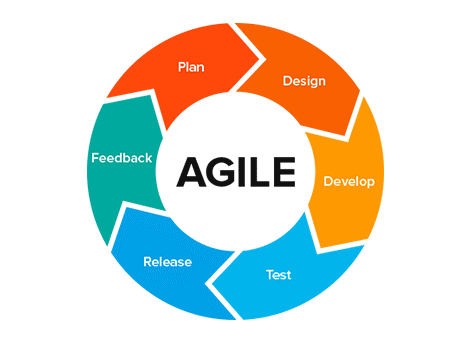
\includegraphics[width=0.75\textwidth]{./img/agile.png}
                \caption{Agile Model for Software Development}
            }
        \end{figure}
        \section{DESCRIPTION OF WORKFLOW}
        \subsection{Data Collection}
        We used dataset created during a Deepfake Image Detection and Reconstruction Challenge.Two datasets of real face images were used: CelebA and FFHQ. Various Deepfake images were generated using architectures such as StarGAN, GDWCT, AttGAN, StyleGAN, and StyleGAN2. Specifically, CelebA images were manipulated using pre-trained models available on GitHub for StarGAN, GDWCT, and AttGAN. Images from StyleGAN and StyleGAN2 created through FFHQ were obtained.
        
        \begin{enumerate}
            \item CelebA\cite{7410782}: A large-scale face attributes dataset containing over 200k celebrity images with 40 labels related to facial attributes such as hair color, gender, and age. The images are in 178 x 218 JPEG format.
            
            \item FFHQ\cite{NVlabs_ffhq_dataset}: A high-quality image dataset of human faces with variations in age, ethnicity, and image background. The images are in 1024 x 1024 PNG format.
            
            \item StarGAN\cite{choi2018stargan}: Capable of performing image-to-image translations on multiple domains using a single model. CelebA images were manipulated with a pre-trained model to achieve a final resolution of 256 x 256.
            
            \item GDWCT\cite{cho2019imagetoimage}: Improves styling capability. CelebA images were manipulated with a pre-trained model to achieve a final resolution of 216 x 216.
    
            \item AttGAN\cite{8718508}: Transfers facial attributes with constraints. CelebA images were manipulated with a pre-trained model to achieve a final resolution of 256 x 256.
        
            \item StyleGAN\cite{Karras_2020_CVPR}: Transfers semantic content from a source domain to a target domain with a different style. Images were generated using FFHQ as the input dataset with a resolution of 1024 x 1024.
        
            \item StyleGAN2\cite{inproceedings}: Improves StyleGAN quality with the same task. Images were generated using FFHQ as the input dataset with a resolution of 1024 x 1024.
        \end{enumerate}
        
        \section{Data Preprocessing}
        \label{sec: above}
        \subsection{Data Augmentation}
            To balance our dataset, we augmented our images to achieve a total of 25000 images for each category. For the 5000 fake images, we applied four different transformations, resulting in 20000 augmented fake images. For the real images, we randomly selected and transformed 3750 images, generating 15000 augmented real images.

            The transformations applied were as follows:
        \begin{enumerate}
            \item Rotation: Images were rotated at an angle randomly selected from [45, 90, 135, 180, 225, 270, 315] degrees.
            \item Mirror: Images were randomly flipped horizontally, vertically, or both.
            \item Scale: Images were randomly scaled at a ratio between [0.5,2].
            \item Compression: Images were compressed using a quality factor between [50,99].
        \end{enumerate}

        After adding the augmented images to the original dataset, we ended up with a total of 25000 real and 25000 fake images.

        \subsection{Data Normalization}
            We first computed the mean and standard deviation of the entire dataset. The normalization was then applied using the formula: 
            \begin{equation}
            x = \frac{x - \mu}{\sigma}
            \end{equation}

        \subsection{Data Splitting}
            We divided our dataset into a training set (80\% of the dataset) and a validation set (20\% of the dataset). This split ensures that the model has a sufficient amount of data to learn from, while also providing a subset of the data to validate the model's performance.


        \section{Implementation}
        
        
        \subsection{CNN}
            A Convolutional Neural Network (CNN) is a Deep Learning algorithm
            that can take in an input image, assign importance (learnable weights and biases) to various aspects/objects in the image, and be able to differentiate one from the other. The pre-processing required in a CNN is much lower as compared to other classification algorithms. While in primitive methods filters are hand-engineered, with enough training, CNNs have the ability to learn these filters characteristics.The architecture of a CNN is analogous to that of the connectivity pattern of Neurons in the Human Brain and was inspired by the organization of the Visual Cortex. Individual neurons respond to stimuli only in a restricted region of the visual field known as the Receptive Field. A collection of such fields overlap to cover the entire visual area.A CNN typically has three layers: a convolutional layer, a pooling layer, and a fully connected layer.

        \begin{figure}[hbt!]
                \center{
                    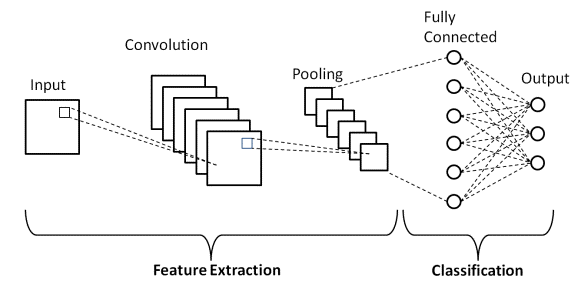
\includegraphics[width=0.9\textwidth]{./img/CNN.png}
                }
                \caption{Convolutional Neural Networks}
        \end{figure}

        \newpage
        \subsection{ResNet}
            ResNet architecture introduced the concept called Residual Blocks. In this network, we use a technique called skip connections. The skip connection connects activations of a  layer to further layers by skipping some layers in between. This forms a residual block. Resnets are made by stacking these residual blocks together. The approach behind this network is instead of layers learning the underlying mapping, we allow the network to fit the residual mapping. So, instead of say H(x), initial mapping, let the network fit,
            \begin{equation}
                F(x) := H(x) - x
            \end{equation}
            which gives
            \begin{equation}
                H(x) := F(x) + x
            \end{equation}
            \begin{figure}[hbt!]
                \center{
                    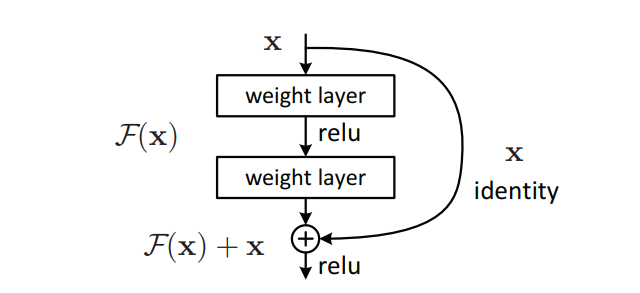
\includegraphics[width=1\textwidth]{./img/ResNet.PNG}
                    \caption{ResNet}
                }
            \end{figure}

        \newpage
        \subsection{Proposed System}
        Below is the representation of our proposed system, illustrated in Figure 4.4. Initially, we assembled the dataset, as outlined in the Data Collection section above. The dataset was categorized into two groups: real and fake. Subsequently, preprocessing of the data was carried out (\ref{sec: above}). For feature extraction and classification, we employed a pre-trained ResNet 9 model. Upon completing the training of the model, it was integrated with a frontend (User Interface) using an API.
        \vspace{20pt}
        \begin{figure}[hbt!]
            \center{
                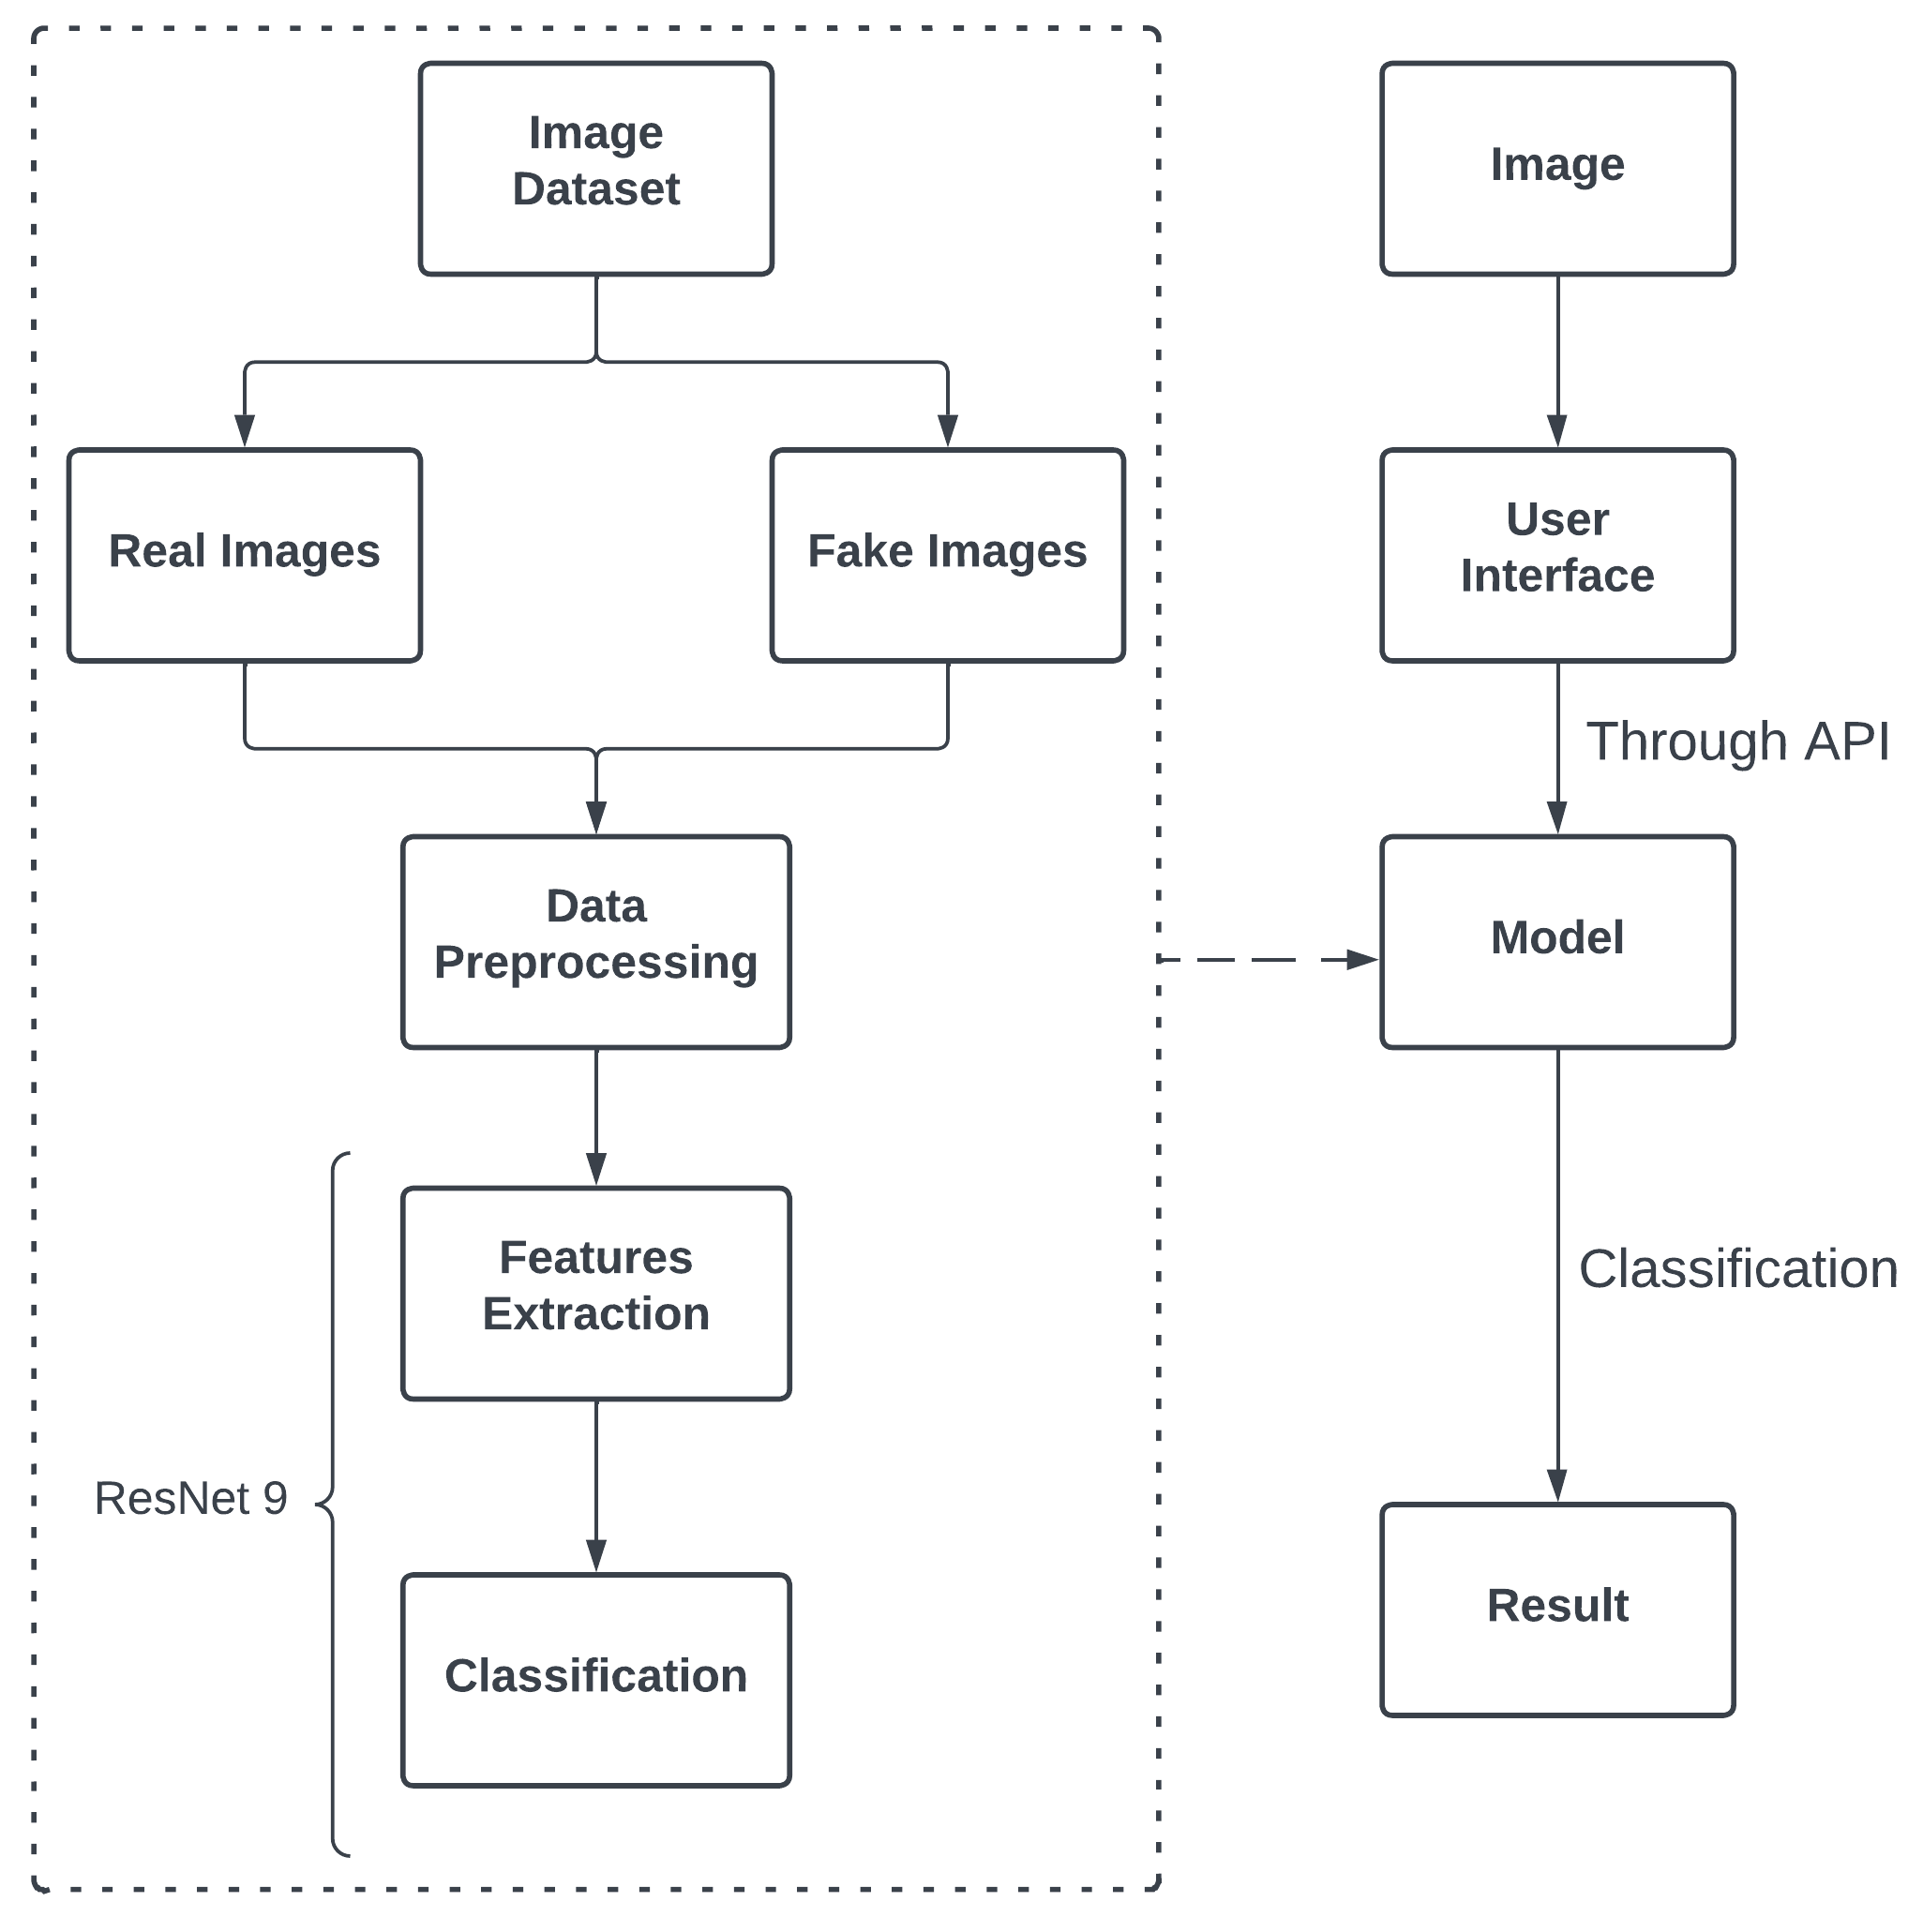
\includegraphics[width=0.65 \textheight]{./img/Implementation Diagram.png}
                \caption{Block Diagram of Proposed System}
            }
        \end{figure}

        % \subsection{GanttChart}
        %     \begin{figure}[hbt!]
        %         \center{
        %             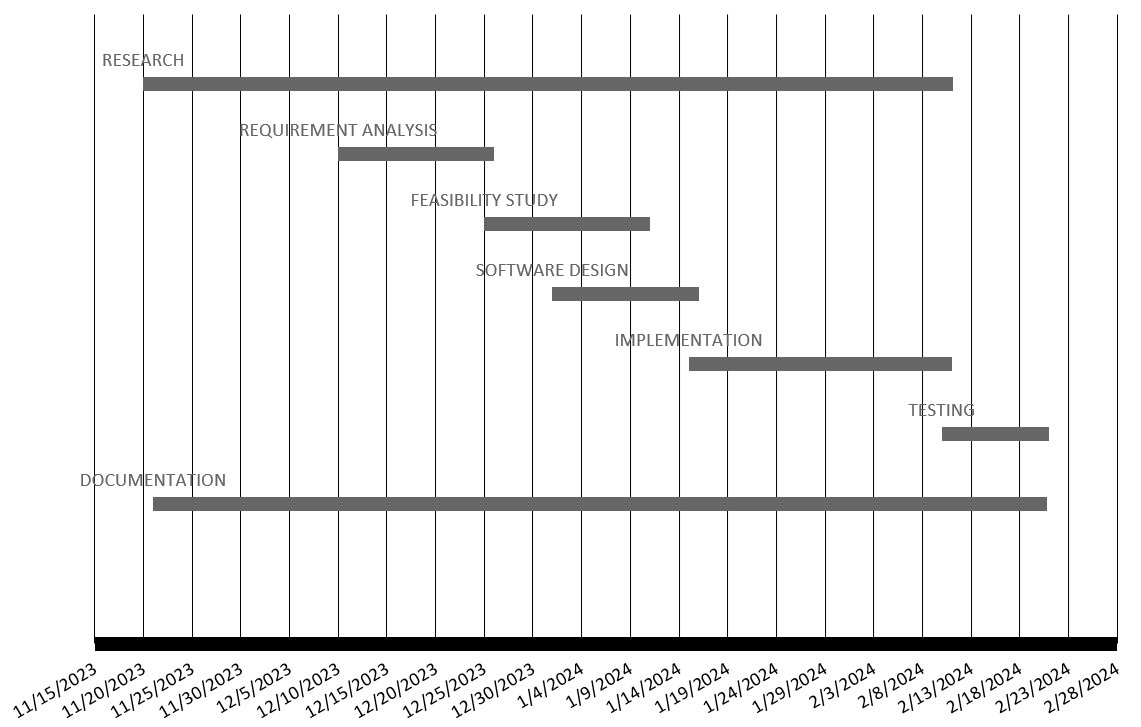
\includegraphics[width=0.1\textwidth]{./img/GANT_CHART.jpg}
        %         }
        %         \caption{Gantt chart}
        %     \end{figure}
